%!TEX root = ../../Main.tex
%!TeX spellcheck = en_US
\graphicspath{{Chapters/2_logistic_regression/}}
%-------------------------------------------------------------------------------

\chapter{Classification}

Classification refers to the practice of predicting qualitative responses. While there are many different classification techniques (also known as classifiers), In this chapter we will touch upon two of the most widely-used ones.

\section{Logistic regression}

Linear regression can be a very useful tool in field of supervised learning, however it requires assumptions that the responds variable $Y$ is quantitative, which often isn't the case. In many contexts, like when discussing eye color, the variable is qualitative, taking on values such blue, green, or brown.

\subsection{Linear vs. Logistic regression}

Why is linearly regression ill suited for cases involving a qualitative responds?

For an example of this, let us consider the case that we are trying to predict which disease a hospital patient has, based on his symptoms. One (simplified) way of encoding this could be

$$\{Rabies,\ Flu,\ Common\ cold,\ Ebola\}$$

However doing this, implies an ordering of the conditions, as well as implying that the the difference between $Flu$ and $Common cold$ is the same as the difference between $Common cold$ and $Ebola$.\\
Furthermore simply changing the ordering of this coding, such as to 

$$\{Flu,\ Rabies,\ Ebola,\ Common\ cold\}$$

Implies a completely different relationship between the conditions. Each separate coding would produce different linear models, each leading to a different set of predictions.

Another problem with using Linear regression, cab be seen by applying it to the data set \texttt{Default}, the result of which can be seen on \cref{fig:LinReg_vs_LogReg}

\begin{figure}[H]
	\fbox{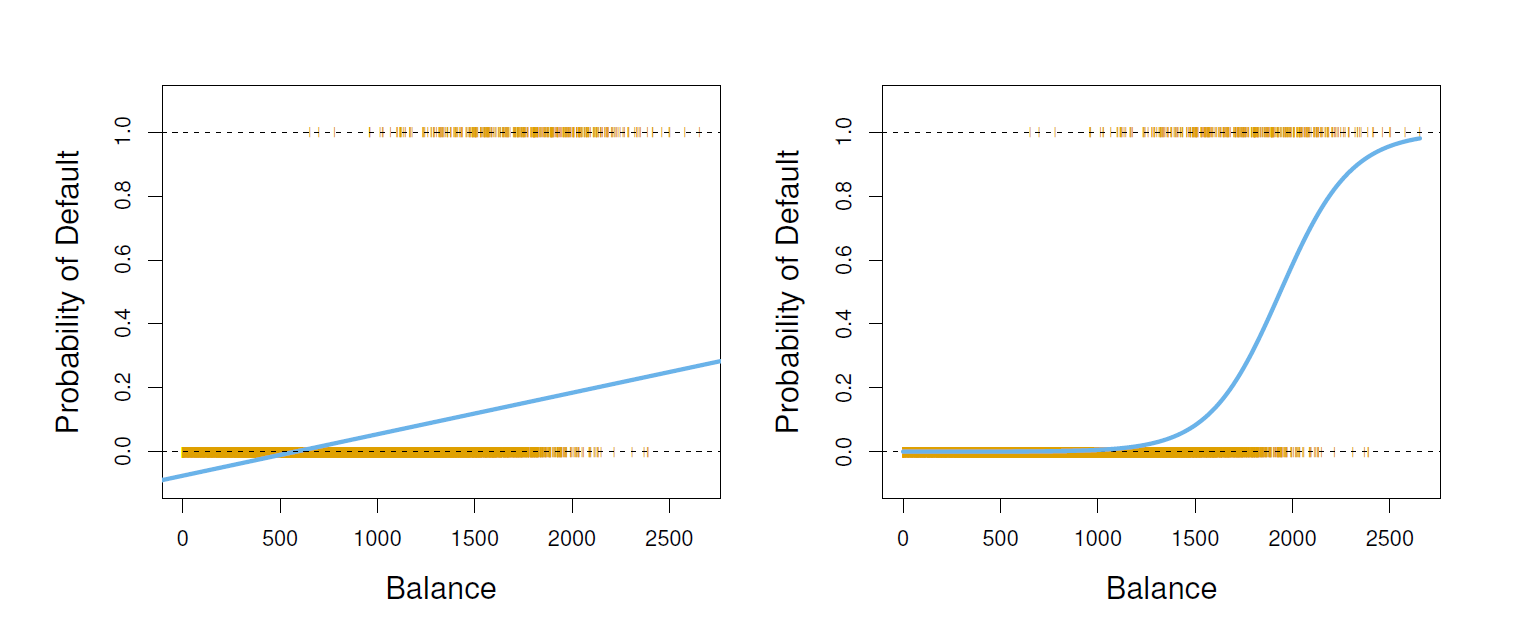
\includegraphics[width=350pt]{Img/LinReg_vs_LogReg}}
	\centering
	\caption{Classification of \texttt{Default} data. Left using linear regression to estimate probability, Right using logistic regression (Source: ISLR book\cite{book_2015} used in DSS course)}
	\label{fig:LinReg_vs_LogReg}
\end{figure}

Here we see that this model estimates some probabilities to be less than 0, and if we were to attempt to predict for a very large balance, we would get a probability greater then 1, neither of these predictions are sensible. Instead we can see the Logistic regression is a much better fit, offering only values between 0 and 1, as well as simply fitting the data more accurately.

\subsection{The logistic model}

In linear regression, we can use the model shown on \cref{eq:LogReg_Linear_Regression_eq} to represent probabilities.

\begin{equation} \label{eq:LogReg_Linear_Regression_eq}
\begin{split}
p(X) & = \beta_0 + \beta_1 X
\end{split}
\end{equation} 

However taking this approach to predict the data on defaulting, ie: $Pr(default=Yes|balance)$, simply yields the model illustrated on the left-hand side of \cref{fig:LinReg_vs_LogReg}. Here we see the problems previously discussed, namely that predictions can be less than 0 and more than 1.

In order to prevent this problem, another model for $p(X)$ must be used, one that guarantees an output between 0 and 1 for all values of $X$. There are numerous functions that can do this, in Logistic regression, the \textbf{logistic function} is used , which can be seen on \cref{eq:LogReg_LogFunc}.

\begin{equation} \label{eq:LogReg_LogFunc}
\begin{split}
p(X)=\frac{e^{\beta_0 + \beta_1 X}}{1+e^{\beta_0 + \beta_1 X}}
\end{split}
\end{equation}



\section{Linear discriminant analysis}

Linear Discriminant analysis is like PCA, but It focuses on maximizing the separability among known categories. This means that LDA makes a line that projects the samples onto it in such a way that it maximizes the separation of these two categories. LDA is used when classes are well separated, and it is also popular when dealing with more than two classes.

\begin{figure}[H]
	\fbox{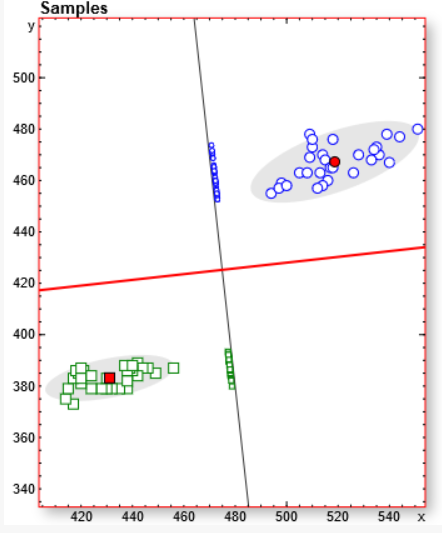
\includegraphics[width=200pt]{Img/LDA_illustration}}
	\centering
	\caption{LDA illustration}
	\label{fig:LDA_illustration}
\end{figure}

On \cref{fig:LDA_illustration} this concept is clearly illustrated and it is easy to see that the samples are well separated onto the (almost) vertical line.

This is done by maximizing the distance between each mean vector of each class and minimizing the variance of each class. On the picture above the red dots are the mean vectors. This is not limited to 2-dimensionel problems and work very well on many-dimensional problems and separates the classes well.